
\chapter{DISEÑO EXPERIMENTO PM-01}
\label{cap:disegno_pm01}

%DESCOMENTAR ESTAS LÍNEAS SI EL CAPÍTULO TIENE FIGURAS O TABLAS
\addtocontents{lof}{{\bf \noindent Figuras del capítulo \arabic{chapter}}}
\addtocontents{lot}{{\bf \noindent Tablas del capítulo \arabic{chapter}}}

En este capítulo se describirán en conjunto los experimentos 1 y 2, que están asociados al PM-01. Esto debido a que gran parte de la estructura general que poseen es similar (como se vio en el capítulo \ref{cap:disegno_experimento}). Las diferencias son especificadas en cada una de las secciones correspondientes.

\section{Estructura de datos}

Los algoritmos generados se construyen en base a varias estructuras de datos. Estas estructuras se diseñaron en base al modelo matemático y a las funciones y terminales que operan sobre ellas. Se dividen en dos clases: estructuras variables y estructuras fijas.

\subsection{Estructura de datos variables}

Las estructuras de datos variables mantienen la información de los ítems que han sido agregados a la mochila y los ítems restantes por agregar. Estas estructuras varían de acuerdo a la acción que realicen los terminales, son las siguientes:

\begin{itemize}
	\item Lista de ítems disponibles (lista de disponibles): lista que contiene todos los ítems disponibles para trabajar en el problema, los ítems pertenecientes a esta lista varían de acuerdo al proceso de la solución. Esta lista se inicializa con todos los ítems disponibles por la instancia del problema.
	\item Lista de ítems ingresados a la mochila (lista de ingresados): lista que contiene todos los ítems agregados a la mochila en algún instante del proceso. Esta lista se encuentra vacía al momento de inicializar el proceso de obtención de la solución.
\end{itemize}

Sobre estas listas solo se pueden realizar dos acciones: agregar un ítem o remover un ítem. Toda acción realizada sobre una de ellas, repercute de forma inversa en la otra. Es decir, si se agrega un ítem en la lista de disponibles, de forma inmediata debe ser removido de la lista de ingresados.

\subsection{Estructura de datos fijas}

Estas estructuras son creadas al momento de iniciar el proceso evolutivo. Son utilizadas por los terminales para poder realizar las acciones que éstos tengan definidas, donde cada una de estas estructuras es inicializada de acuerdo a los valores que se obtienen de las instancias. Las estructuras de datos fijas pueden estar contenidas dentro de las estructuras de datos variables. A continuación, se presenta el detalle de éstas:

\begin{itemize}
	\item Capacidad de la mochila: contiene el valor del tamaño máximo de ítems que puede soportar la mochila.
	\item Valor óptimo de la instancia: contiene el valor óptimo del beneficio de la instancia.
	\item Datos de cada ítem: lista que contiene todos los datos de la mochila. Estos datos son: número del ítem, beneficio del ítem, peso del ítem, ganancia del ítem ($\dfrac{beneficio}{peso}$). Los valores son inicializados al momento de cargar la instancia para cada uno de los ítems disponibles en ésta y posteriormente agregado a la lista de disponibles. Cada uno de estos ítems con sus respectivos datos es invariable en el transcurso del proceso evolutivo.
\end{itemize}

\section{Funciones y terminales}

Las funciones y terminales son las operaciones elementales sobre las estructuras de datos anteriormente definidas. Por lo tanto, su definición es fundamental para generar algoritmos con la capacidad de utilizar estas estructuras con el fin de alcanzar una solución que aumente el beneficio de los ítems en la mochila. Se construyen terminales en base a heurísticas existentes para el PM-01, y funciones que permitan operar en diversas combinaciones sobre estos terminales.

Los elementos del conjunto de funciones y terminales deben cumplir con las propiedades de suficiencia y clausura \citep{poli_2008}. Las funciones y terminales cumplen la propiedad de clausura, ya que todas retornan un valor verdadero o falso, y las funciones solo pueden recibir parámetros de entrada de ese tipo. La propiedad de suficiencia se cumple con cada uno de los terminales, ya que éstos se encargan de agregar o retirar ítems de la mochila, adicionalmente cualquier estado de la mochila es una solución factible, aunque esté vacía.

\subsection{Conjunto de funciones}

Las funciones que conforman los algoritmos generados contienen instrucciones básicas utilizadas en su mayoría por todos los lenguajes de programación. Desde el punto de vista de la PG, las funciones corresponden a los nodos internos del árbol \citep{koza_poli_2005}. Estas se listan en la Tabla \ref{tab:func_pm01}.

\begin{table}[hbtp!]
\caption{Grupo de funciones para el PM-01.}\label{tab:func_pm01}
\small
\centering
\rowcolors{2}{gray!25}{white}
\begin{tabular}{ccl}
\hline
{\textbf{Nº}} & {\textbf{Nombre}} & {\textbf{Descripción}} \\ \hline
1	& $while(A, B)$				&	\begin{tabular}[c]{@{}l@{}}
										Mientras la expresión A sea Verdadera se ejecuta la instrucción B. \\
										Tiene como límite de iteraciones que el valor del beneficio no varíe \\
										en tres iteraciones.\\ 
										Devuelve verdadero en caso de realizar una o más iteraciones y \\
										falso en caso contrario.
									\end{tabular} \\
2	& $IfThenElse(A, B, C)$		&	\begin{tabular}[c]{@{}l@{}}
										Ejecuta B si A es verdadero y C si A es falso. \\
										Devuelve el valor de B o C según sea el caso.
									\end{tabular} \\
3	& $IfThen(A, B)$			&	\begin{tabular}[c]{@{}l@{}}
										Ejecuta B si A es verdadero.\\
										Devuelve verdadero si logra ejecutar B al menos una vez y \\
										devuelve falso en caso contrario.
									\end{tabular} \\
4	& $Not(A)$					&	\begin{tabular}[c]{@{}l@{}}
										Función lógica que implementa la negación lógica. \\
										Devuelve verdadero si A es falso y devuelve falso si A \\
										es verdadero.
									\end{tabular} \\
5	& $And(A, B)$				&	\begin{tabular}[c]{@{}l@{}}
										Función lógica que implementa la conjunción lógica. \\
										Devuelve verdadero si A y B son verdaderos y devuelve falso \\
										en los otros casos.
									\end{tabular} \\
6	& $Or(A, B)$				&	\begin{tabular}[c]{@{}l@{}}
										Función lógica que implementa la disyunción lógica. \\
										Devuelve verdadero si A o B son verdaderos y devuelve falso \\
										en los otros casos.
									\end{tabular} \\
7	& $Equal(A, B)$				&	\begin{tabular}[c]{@{}l@{}}
										Función que compara la igualdad de A y B. \\
										Devuelve verdadero si A y B son iguales y devuelve falso \\
										en caso contrario.
									\end{tabular} \\
\hline
\end{tabular}
\caption*{(Elaboración propia, 2015)}
\end{table}

\subsection{Conjunto de terminales}

Los terminales son funciones diseñadas para el PM-01, los que permiten agregar o quitar ítems de la mochila de acuerdo a algún criterio establecido. De acuerdo a la definición de la PG, un terminal es un nodo hoja \citep{koza_poli_2005}. Cada uno de los terminales es una heurística elemental capaz de modificar la estructura de datos definida generando nuevas soluciones. Se ha restringido los terminales para que no puedan generar soluciones infactibles para el problema, es decir, no es posible generar soluciones que no cumplan alguna de las restricciones propias problema. Los terminales a utilizar son los utilizados por Parada \citep{parada_2015}, éstos son descritos en la Tabla \ref{tab:term_pm01}.

\begin{table}[htbp!]
\caption{Grupo de terminales para el PM-01.}\label{tab:term_pm01}
\small
\centering
\rowcolors{2}{gray!25}{white}
\begin{tabular}{ccl}
\hline
{\textbf{Nº}} & {\textbf{Nombre}} & {\textbf{Descripción}} \\ \hline
1	& AgregarMasPesado			&	\begin{tabular}[c]{@{}l@{}}
										Busca el ítem con mayor peso dentro de la lista de \\
										disponibles. Si encuentra un ítem, verifica si puede \\
										agregarlo a la lista de ingresados y lo elimina de la \\
										lista de disponibles. \\
										Si logra ingresar el ítem a la lista de disponibles \\
										retorna verdadero, sino retorna falso.
									\end{tabular} \\
2	& AgregarMenosPesado		&	\begin{tabular}[c]{@{}l@{}}
										Busca el ítem con menor peso dentro de la lista de \\
										disponibles. Si encuentra un ítem, verifica si puede \\
										agregarlo a la lista de ingresados y lo elimina de la \\
										lista de disponibles. \\
										Si logra ingresar el ítem a la lista de disponibles \\
										retorna verdadero, sino retorna falso.
									\end{tabular} \\
3	& AgregarPrimeroDisponible	&	\begin{tabular}[c]{@{}l@{}}
										Verifica si el primer ítem de la lista de disponible \\
										puede ser agregado a la mochila y lo elimina de la lista \\
										de disponibles. \\
										Si logra ingresar el ítem a la lista de disponibles \\
										retorna verdadero, sino retorna falso.
									\end{tabular} \\
4	& AgregarMayorBeneficio		&	\begin{tabular}[c]{@{}l@{}}
										Busca el ítem con mayor beneficio dentro de la lista \\
										de disponibles. Si encuentra un ítem, verifica si puede \\
										agregarlo a la lista de ingresados y lo elimina de la \\
										lista de disponibles. \\
										Si logra ingresar el ítem a la lista de disponibles \\
										retorna verdadero, sino retorna falso.
									\end{tabular} \\
5	& AgregarMenorBeneficio		&	\begin{tabular}[c]{@{}l@{}}
										Busca el ítem con menor beneficio dentro de la lista \\
										de disponibles. Si encuentra un ítem, verifica si puede \\
										agregarlo a la lista de ingresados y lo elimina de la \\
										lista de disponibles. \\
										Si logra ingresar el ítem a la lista de disponibles \\
										retorna verdadero, sino retorna falso.
									\end{tabular} \\
6	& AgregarMayorGanancia		&	\begin{tabular}[c]{@{}l@{}}
										Busca el ítem con mayor ganancia (beneficio / peso) dentro \\
										de la lista de disponibles. Si encuentra un ítem, verifica \\
										si puede agregarlo a la lista de ingresados y lo elimina de \\
										la lista de disponibles. \\
										Si logra ingresar el ítem a la lista de disponibles retorna \\
										verdadero, sino retorna falso.
									\end{tabular} \\
\hline
\end{tabular}
\caption*{(Elaboración propia, 2015)}
\end{table}

\addtocounter{table}{-1}
\begin{table}[htbp!]
\caption{Grupo de terminales para el PM-01 (continuación).}\label{tab:term_pm01_2}
\small
\centering
\rowcolors{2}{gray!25}{white}
\begin{tabular}{ccl}
\hline
{\textbf{Nº}} & {\textbf{Nombre}} & {\textbf{Descripción}} \\ \hline
7	& AgregarMenorGanancia		&	\begin{tabular}[c]{@{}l@{}}
										Busca el ítem con menor ganancia (beneficio / peso) dentro \\
										de la lista de disponibles. Si encuentra un ítem, verifica \\
										si puede agregarlo a la lista de ingresados y lo elimina de \\
										la lista de disponibles. \\
										Si logra ingresar el ítem a la lista de disponibles retorna \\
										verdadero, sino retorna falso.
									\end{tabular} \\
8	& IsFull					&	\begin{tabular}[c]{@{}l@{}}
										Retorna verdadero si la mochila está llena, retorna \\
										falso en caso contrario.
									\end{tabular} \\
9	& IsTrue					&	\begin{tabular}[c]{@{}l@{}}
										Retorna verdadero.
									\end{tabular} \\
10	& EliminarMasPesado			&	\begin{tabular}[c]{@{}l@{}}
										Busca el ítem con mayor peso dentro de la lista de \\
										ingresados. Si encuentra un ítem lo elimina de lista de \\
										ingresados y lo agrega a la lista de disponibles. \\
										Si logra eliminar el ítem a la lista de ingresados retorna \\
										verdadero, sino retorna falso.
									\end{tabular} \\
11	& EliminarPeorBeneficio		&	\begin{tabular}[c]{@{}l@{}}
										Busca el ítem con peor beneficio dentro de la lista de \\
										ingresados. Si encuentra un ítem lo elimina de lista de \\
										ingresados y lo agrega a la lista de disponibles. \\
										Si logra eliminar el ítem a la lista de ingresados retorna \\
										verdadero, sino retorna falso.
									\end{tabular} \\
12	& EliminarPeorGanancia		&	\begin{tabular}[c]{@{}l@{}}
										Busca el ítem con peor ganancia (beneficio / peso) dentro de \\
										la lista de ingresados. Si encuentra un ítem lo elimina de \\
										lista de ingresados y lo agrega a la lista de disponibles. \\
										Si logra eliminar el ítem a la lista de ingresados retorna \\
										verdadero, sino retorna falso.
									\end{tabular} \\
\hline
\end{tabular}
\caption*{(Elaboración propia, 2015)}
\end{table}

\section{Función de evaluación}
\label{cap:func_eval_pm01}

La función de evaluación es el mecanismo primario para comunicar la declaración de alto nivel de los requisitos del problema con el sistema de PG \citep{koza_poli_2005}. En el capítulo \ref{cap:disegno_experimento} se describe la diferencia que presentan las funciones de evalución de los experimentos 1 y 2. En el caso de la PG tradicional, se utiliza una función de evaluación compuesta por las dos funciones de evaluación utilizadas en el caso de las islas. La función de evaluación para el experimento tiene por objetivo medir la calidad de los algoritmos y su legibilidad desde el punto de vista de un humano. La calidad está dada por “que tan bien resuelve el algoritmo el problema”, es decir, que tan “cerca” estoy del valor óptimo. La legibilidad está dada por “que tan fácil es leer, entender y ejecutar el algoritmo por un humano”. La estructura de los algoritmos generados es representada por nodos de un árbol sintáctico, siendo estos nodos los terminales y funciones. Mientras menor sea la cantidad de nodos es más fácil leer el algoritmo representado por el árbol sintáctico. Por lo tanto, la legibilidad de un algoritmo se considera como opuesta al tamaño de éste.

La calidad de los algoritmos es el factor que varía entre las distintas funciones objetivo de los experimentos, mientras que la legibilidad es una función común a todos los casos. Esta función de legibilidad $leg_{p}$ para el algoritmo $p$ está dada la ecuación (\ref{eq:leg_pm01}). Donde $N_{p}$ es el número de nodos del algoritmo $p$, mientras que $M_{p}$ es el número máximo de nodos permitidos para los algoritmos.

\begin{equation}
\label{eq:leg_pm01}
	leg_{p} = 	\begin{cases}
					0       & \quad \text{si } N_{p} \leq M_{p} \\
					\frac{M_{p}-N_{p}}{M_{p}}  & \quad \text{si } N_{p} > M_{p}\\
				\end{cases}
\end{equation}

\subsection{Función de evaluación experimento con co-evolución}
\label{cap:fo_coev}

Para el experimento con co-evolución durante el proceso evolutivo se requieren dos funciones de evaluación que cumplan con evaluar la calidad de los algoritmos de acuerdo al problema. Para esto se utilizan las siguientes funciones de evaluación.

Función de evaluación de la calidad por medio del ERP: como se mencionó en las secciones \ref{cap:experimento_tradicional} y \ref{cap:experimento_islas}, el ERP consiste en el error relativo promedio de los algoritmos obtenidos. Para cada grupo de instancias de evaluación $S$, se determina el porcentaje promedio por el cual el beneficio obtenido $o_{i}$ se encuentra distanciado de la mejor solución $z_{i}$ para cada instancia del conjunto $S$. Esto se representa en la ecuación (\ref{eq:ERP_pm01}), donde $n_{s}$ representa el número de instancias del conjunto $S$.

\begin{equation}
\label{eq:ERP_pm01}
	ERP_{s} =  \frac{1}{n_{s}} \cdot \sum\limits_{i=1}^{n_{s}} \frac{z_{i} - o_{i}}{z_{i}} 
\end{equation}

Función de evaluación de la calidad por medio de los HITS: esta función de evaluación representa que tantas instancias $i$ del conjunto $S$ evaluadas con el algoritmo $p$ obtienen un error relativo menor a $0,01$ ($1\%$). La ecuación (\ref{eq:ER_pm01}) representa el ER de la instancia $i$, el cual es utilizado en la ecuación (\ref{eq:HIT_pm01}) para determinar si el resultado de éste es $1$ o $0$. Finalmente la ecuación (\ref{eq:HITS_pm01}) utiliza los resultados obtenidos en la evaluación de cada una de las instancias $i$ por la ecuación (\ref{eq:HIT_pm01}) para calcular el número de \textit{hits} (aciertos) que obtiene el algoritmo $p$.

\begin{equation}
\label{eq:ER_pm01}
	ER_{i} = \frac{z_{i}-o{i}}{z_{i}}
\end{equation}

\begin{equation}
\label{eq:HIT_pm01}
	HIT_{i} = 	\begin{cases}
					1       & \quad \text{si } ER_{i} \leq 1\% \\
					0  		& \quad \text{si } ER_{i} > 1\%	   \\
				\end{cases}
\end{equation}

\begin{equation}
\label{eq:HITS_pm01}
	HITS_{s} = \frac{n_{s} - \sum\limits_{i=1}^{n_{s}} HIT_{i} }{n_{s}}
\end{equation}

Finalmente, las funciones de evaluación de calidad representadas en las ecuaciones (\ref{eq:ERP_pm01}) y (\ref{eq:HITS_pm01}) se les debe agregar el factor de legibilidad representado por la ecuación (\ref{eq:leg_pm01}). Como se menciona en la sección \ref{cap:func_eval_pm01} el factor de legibilidad representa una menor relevancia que el de las funciones de evaluación, por lo que se utiliza un factor de relevancia $\alpha$ y $\beta=(1 - \alpha)$. En las ecuaciones (\ref{eq:fo1_islas_pm01}) y (\ref{eq:fo2_islas_pm01}) se representa la función de evaluación 1 y función de evaluación 2, respectivamente para el experimento 2.

\begin{equation}
\label{eq:fo1_islas_pm01}
	fe_{1} = \alpha\cdot ERP_{s}+ \beta\cdot leg_{p}
\end{equation}

\begin{equation}
\label{eq:fo2_islas_pm01}
	fe_{2} = \alpha\cdot HITS_{s}+ \beta\cdot leg_{p}
\end{equation}

\subsection{Función de evaluación experimento sin co-evolución}
\label{cap:fo_trad}

Para el experimento sin co-evolución o tradicional, durante el proceso evolutivo se utiliza una función de evaluación combinada de las funciones de evaluación representadas en las ecuaciones (\ref{eq:ERP_pm01}) y (\ref{eq:HITS_pm01}) de acuerdo a lo mencionado en la sección \ref{cap:experimento_islas}. La ecuación (\ref{eq:comb_trad_pm01}) representa la combinación de las ecuaciones mencionadas.

\begin{equation}
\label{eq:comb_trad_pm01}
	fe_{pm-01} = \alpha\cdot ERP_{s}+ \beta\cdot HITS_{s}
\end{equation}

Al igual que en la sección \ref{cap:fo_coev} a la ecuación (\ref{eq:comb_trad_pm01}) es necesario agregarle el factor de legibilidad de la ecuación (\ref{eq:leg_pm01}), resultando la ecuación (\ref{eq:fo_trad_pm01}).

\begin{equation}
\label{eq:fo_trad_pm01}
	fe = \alpha\cdot(\alpha\cdot ERP_{s}+ \beta\cdot HITS_{s}) + \beta\cdot leg_{p}
\end{equation}

\section{Selección casos de adaptación}
\label{cap:sel_casos_adapt_pm01}

Los casos de adaptación (instancias) para el problema, fueron producidos usando un generador aleatorio de problemas desarrollado por Pisinger \citep{pisinger_2005}. El generador permite producir instancias con distintos rangos de distribución de $w_{j}/p_{j}$, a partir de lo cual son clasificados siete grupos de instancias clásicas: no correlacionadas (NC), débilmente correlacionadas (DC), fuertemente correlacionadas (FC), inversamente fuertemente correlacionadas (IFC), semi-fuertemente correlacionadas (SFC), suma de sub-conjuntos (SS) y no correlacionadas con igual peso (NCSW). De estos grupos se escogen las NC, DC, FC, SS, siendo las más distintas dentro de la clasificación. Esto debido a que según menciona Pisinger \citep{pisinger_2005}, algunas de estas clasificaciones son muy similares, produciendo poco “ruido” en la diferencia entre ellas. Adicionalmente, Pisinger propone una clasificación con nuevos casos de estudio, decidiendo de forma arbitraria utilizar las instancias con denominadas \textit{“profit ceiling instances pceil(3)”} (\textit{Ceil}) para agregar mayor variabilidad a las instancias de los grupos anteriores. La distribución de la relación entre el beneficio y peso de cada ítem se muestra en la Figura \ref{fig:correlaciones}. En esta Figura se presentan los grupos a utilizar, donde cada uno de los gráficos muestra la distribución del beneficio y peso de cada ítem que posee cada grupo.

\begingroup
    \centering
    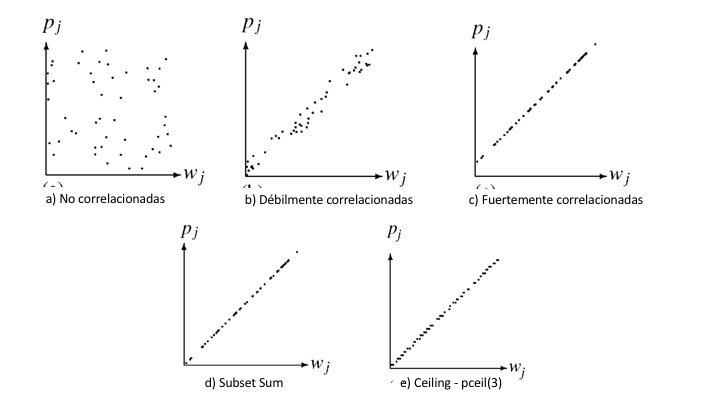
\includegraphics[width=14cm]{images/cap3/correlaciones.jpg}
    \captionof{figure}{Relación entre peso y beneficio de los ítems de la mochila para cada grupo \citep{pisinger_2005}.}\label{fig:correlaciones}
\endgroup

El conjunto de instancias disponibles cuenta con un total de 792 instancias para cada uno de los grupos a utilizar (3960 instancias en total para los cinco grupos mencionados), las que varían entre 50, 100, 200, 500, 1000, 2000, 5000 y 10.000 ítems por instancia de una forma equitativamente distribuida. Es decir, el grupo NC cuenta con 99 instancias que contienen 50 ítems, 99 instancias que contienen 100 ítems, 99 instancias que contienen 200 ítems, 99 instancias que contienen 500 ítems, 99 instancias que contienen 1.000 ítems, 99 instancias que contienen 2.000 ítems, 99 instancias que contienen 5.000 ítems y 99 instancias que contienen 10.000 ítems, y así sucesivamente para cada uno de los grupos. Todas las instancias disponibles cuentan con su valor óptimo y a lo menos una posible solución. Estas instancias pueden ser encontradas en \url{http://www.diku.dk/~pisinger/codes.html}.

Dada la gran cantidad de casos de adaptación, se realiza un experimento utilizando cada uno de los grupos seleccionados, más la adición de un grupo que contenga la mezcla de los demás (GX). Es decir, se realizan seis sub-experimentos dentro de cada uno de los experimentos del PM-01. Estos experimentos utilizan los grupos NC, DC, FC, SS, Ceil y GX, tanto para el experimento 1 como el experimento 2. 

Del total de instancias se ha seleccionado un grupo como caso de adaptación para el proceso evolutivo y otro grupo como evaluación de los algoritmos generados en el proceso evolutivo. Las instancias a evaluar fueron generadas de forma automática con el mismo criterio para cada uno de los grupos descritos, por lo que la selección de instancias utilizadas para cada grupo (evolución y evaluación) es determinada de forma arbitraria. En los casos de adaptación, el número de instancias varía de acuerdo a cada uno de los experimentos 1 y 2, ya que como se mencionó en el capítulo \ref{cap:disegno_experimento}, las instancias es otro factor que varía para el diseño de éstos. El tamaño de las instancias (cantidad de ítems) para los casos de adaptación varía entre 50, 100, 200, 500. Este tamaño del problema claramente una complejidad alta para un experto humano y permite ejecutar la PG en tiempos razonables. Para las instancias de evaluación son utilizados los mismos grupos para ambos experimentos.


\subsection{Conjuntos de instancias de adaptación con co-evolución}
\label{cap:ins_coev}

Para el experimento con co-evolución durante el proceso evolutivo se requieren dos conjuntos de instancias de adaptación. Estos grupos de instancias son diferenciados por su tamaño. Para el grupo 1 se utilizan las instancias de tamaño 200 y 500, mientras que para el grupo 2 se utilizan instancias de tamaño 50 y 100. El número de instancias para cada grupo es de seis instancias, siendo tres de cada uno de los tamaños mencionados. Este número ha sido determinado en trabajos relacionados \citep{contreras_2013, parada_2015} y permite obtener buenos resultados para el proceso evolutivo. En la Tabla \ref{tab:ins_islas} se encuentran las instancias de adaptación para cada uno de los casos. En éstas se puede apreciar que el grupo GX está compuesta por algunas de las instancias pertenecientes a los otros grupos. Por otra parte, las instancias son clasificadas por el nombre del grupo y un correlativo correspondiente a la pertenencia que tengan a los grupos 1 o 2 de instancias. Por ejemplo, NC1 pertenece al grupo NC de clasificación y al grupo 1 de las instancias.

\begin{table}[hbtp!]
\caption{Conjunto de instancias de adaptación para el experimento 2}\label{tab:ins_islas}
\small
\centering
\begin{center}
\begin{tabular}{cc||ccc}
\hline
{\textbf{Grupo}} & {\textbf{Nombre instancia}} & {\textbf{Grupo}} & \multicolumn{2}{c}{{\textbf{Nombre instancia}}} \\ \hline
NC1 & 	\begin{tabular}[c]{@{}l@{}}
						 knapPI\_1\_200\_1000\_26 \\ 
						 knapPI\_1\_200\_1000\_63 \\
						 knapPI\_1\_200\_1000\_8 \\
						 knapPI\_1\_500\_1000\_5 \\
						 knapPI\_1\_500\_1000\_86 \\
						 knapPI\_1\_500\_1000\_94
						\end{tabular} & DC1 & 
										\multicolumn{2}{c}{
											\begin{tabular}[c]{@{}l@{}}
											 knapPI\_2\_200\_1000\_26 \\
											 knapPI\_2\_200\_1000\_63 \\
											 knapPI\_2\_200\_1000\_8 \\
											 knapPI\_2\_500\_1000\_5 \\
											 knapPI\_2\_500\_1000\_86 \\
											 knapPI\_2\_500\_1000\_94
											\end{tabular}}\\
\hline
NC2 & 	\begin{tabular}[c]{@{}l@{}}
						 knapPI\_1\_100\_1000\_19 \\
						 knapPI\_1\_100\_1000\_26 \\
						 knapPI\_1\_100\_1000\_6 \\
						 knapPI\_1\_50\_1000\_19 \\
						 knapPI\_1\_50\_1000\_26 \\
						 knapPI\_1\_50\_1000\_7 
						\end{tabular} & DC2 &
										\multicolumn{2}{c}{
											\begin{tabular}[c]{@{}l@{}}
											 knapPI\_2\_100\_1000\_19 \\
											 knapPI\_2\_100\_1000\_26 \\
											 knapPI\_2\_100\_1000\_6 \\
											 knapPI\_2\_50\_1000\_19 \\
											 knapPI\_2\_50\_1000\_26 \\
											 knapPI\_2\_50\_1000\_7 
											\end{tabular}}\\
\hline
FC1 & 	\begin{tabular}[c]{@{}l@{}}
						 knapPI\_3\_200\_1000\_26 \\
						 knapPI\_3\_200\_1000\_63 \\
						 knapPI\_3\_200\_1000\_8 \\
						 knapPI\_3\_500\_1000\_5 \\
						 knapPI\_3\_500\_1000\_86 \\
						 knapPI\_3\_500\_1000\_94 
						\end{tabular} & SS1 &
										\multicolumn{2}{c}{
											\begin{tabular}[c]{@{}l@{}}
											 knapPI\_6\_200\_1000\_26 \\
											 knapPI\_6\_200\_1000\_63 \\
											 knapPI\_6\_200\_1000\_8 \\
											 knapPI\_6\_500\_1000\_5 \\
											 knapPI\_6\_500\_1000\_86 \\
											 knapPI\_6\_500\_1000\_94 
											\end{tabular}}\\
\hline
FC2 & 	\begin{tabular}[c]{@{}l@{}}
						 knapPI\_3\_100\_1000\_19 \\
						 knapPI\_3\_100\_1000\_26 \\
						 knapPI\_3\_100\_1000\_6 \\
						 knapPI\_3\_50\_1000\_19 \\
						 knapPI\_3\_50\_1000\_26 \\
						 knapPI\_3\_50\_1000\_7 
						\end{tabular} & SS2 & 
										\multicolumn{2}{c}{				
											\begin{tabular}[c]{@{}l@{}}
											 knapPI\_6\_100\_1000\_19 \\
											 knapPI\_6\_100\_1000\_26 \\
											 knapPI\_6\_100\_1000\_6 \\
											 knapPI\_6\_50\_1000\_19 \\
											 knapPI\_6\_50\_1000\_26 \\
											 knapPI\_6\_50\_1000\_7 
											\end{tabular}}\\
\hline
Ceil1 & 	\begin{tabular}[c]{@{}l@{}}
							 knapPI\_15\_200\_1000\_26 \\
							 knapPI\_15\_200\_1000\_63 \\
							 knapPI\_15\_200\_1000\_8 \\
							 knapPI\_15\_500\_1000\_5 \\
							 knapPI\_15\_500\_1000\_86 \\
							 knapPI\_15\_500\_1000\_94
							\end{tabular} & GX1 &  \begin{tabular}[c]{@{}l@{}}
																		 knapPI\_1\_200\_1000\_8 \\
																		 knapPI\_2\_200\_1000\_8 \\
																		 knapPI\_3\_200\_1000\_8 \\
																		 knapPI\_6\_200\_1000\_8 \\
																		 knapPI\_15\_200\_1000\_8
																	\end{tabular} &  \begin{tabular}[c]{@{}l@{}}
																		 knapPI\_1\_500\_1000\_5 \\
																		 knapPI\_2\_500\_1000\_5 \\
																		 knapPI\_3\_500\_1000\_5 \\
																		 knapPI\_6\_500\_1000\_5 \\
																		 knapPI\_15\_500\_1000\_5
																	\end{tabular}\\ 
\hline
Ceil2 & 	\begin{tabular}[c]{@{}l@{}}
							 knapPI\_15\_100\_1000\_19 \\
							 knapPI\_15\_100\_1000\_26 \\
							 knapPI\_15\_100\_1000\_6 \\
							 knapPI\_15\_50\_1000\_19 \\
							 knapPI\_15\_50\_1000\_26 \\
							 knapPI\_15\_50\_1000\_7 
							\end{tabular} & GX2 &  \begin{tabular}[c]{@{}l@{}}
																		 knapPI\_1\_100\_1000\_6 \\
																		 knapPI\_2\_100\_1000\_6 \\
																		 knapPI\_3\_100\_1000\_6 \\
																		 knapPI\_6\_100\_1000\_6 \\
																		 knapPI\_15\_100\_1000\_6
																	\end{tabular} &  \begin{tabular}[c]{@{}l@{}}
																		 knapPI\_1\_50\_1000\_7 \\
																		 knapPI\_2\_50\_1000\_7 \\
																		 knapPI\_3\_50\_1000\_7 \\
																		 knapPI\_6\_50\_1000\_7 \\
																		 knapPI\_15\_50\_1000\_7
																	\end{tabular}\\ 
\hline
\end{tabular}
\end{center}
\caption*{(Elaboración propia, 2015)}
\end{table}


\subsection{Conjuntos de instancias de adaptación sin co-evolución}

El conjunto de instancias de adaptación para el experimento sin co-evolución es la combinación de los grupos 1 y 2 utilizados en \ref{cap:ins_coev} para cada uno de los grupos. En la Tabla \ref{tab:ins_trad} se puede apreciar los grupos y sus respectivas instancias.

\begin{table}[hbtp!]
\caption{Conjunto de instancias de adaptación para el experimento 1}\label{tab:ins_trad}
\small
\centering
\begin{center}
\begin{tabular}{cc||ccc}
\hline
{\textbf{Grupo}} & {\textbf{Nombre instancia}} & {\textbf{Grupo}} & \multicolumn{2}{c}{{\textbf{Nombre instancia}}} \\ \hline
NC & 	\begin{tabular}[c]{@{}l@{}}
						 knapPI\_1\_200\_1000\_26 \\ 
						 knapPI\_1\_200\_1000\_63 \\
						 knapPI\_1\_200\_1000\_8 \\
						 knapPI\_1\_500\_1000\_5 \\
						 knapPI\_1\_500\_1000\_86 \\
						 knapPI\_1\_500\_1000\_94 \\
						 knapPI\_1\_100\_1000\_19 \\
						 knapPI\_1\_100\_1000\_26 \\
						 knapPI\_1\_100\_1000\_6 \\
						 knapPI\_1\_50\_1000\_19 \\
						 knapPI\_1\_50\_1000\_26 \\
						 knapPI\_1\_50\_1000\_7
						\end{tabular} & DC & 
										\multicolumn{2}{c}{
											\begin{tabular}[c]{@{}l@{}}
											 knapPI\_2\_200\_1000\_26 \\
											 knapPI\_2\_200\_1000\_63 \\
											 knapPI\_2\_200\_1000\_8 \\
											 knapPI\_2\_500\_1000\_5 \\
											 knapPI\_2\_500\_1000\_86 \\
											 knapPI\_2\_500\_1000\_94 \\
											 knapPI\_2\_100\_1000\_19 \\
											 knapPI\_2\_100\_1000\_26 \\
											 knapPI\_2\_100\_1000\_6 \\
											 knapPI\_2\_50\_1000\_19 \\
											 knapPI\_2\_50\_1000\_26 \\
											 knapPI\_2\_50\_1000\_7 
											\end{tabular}}\\

\hline
FC & 	\begin{tabular}[c]{@{}l@{}}
						 knapPI\_3\_200\_1000\_26 \\
						 knapPI\_3\_200\_1000\_63 \\
						 knapPI\_3\_200\_1000\_8 \\
						 knapPI\_3\_500\_1000\_5 \\
						 knapPI\_3\_500\_1000\_86 \\
						 knapPI\_3\_500\_1000\_94 \\
						 knapPI\_3\_100\_1000\_19 \\
						 knapPI\_3\_100\_1000\_26 \\
						 knapPI\_3\_100\_1000\_6 \\
						 knapPI\_3\_50\_1000\_19 \\
						 knapPI\_3\_50\_1000\_26 \\
						 knapPI\_3\_50\_1000\_7 
						\end{tabular} & SS &
										\multicolumn{2}{c}{
											\begin{tabular}[c]{@{}l@{}}
											 knapPI\_6\_200\_1000\_26 \\
											 knapPI\_6\_200\_1000\_63 \\
											 knapPI\_6\_200\_1000\_8 \\
											 knapPI\_6\_500\_1000\_5 \\
											 knapPI\_6\_500\_1000\_86 \\
											 knapPI\_6\_500\_1000\_94 \\
											 knapPI\_6\_100\_1000\_19 \\
											 knapPI\_6\_100\_1000\_26 \\
											 knapPI\_6\_100\_1000\_6 \\
											 knapPI\_6\_50\_1000\_19 \\
											 knapPI\_6\_50\_1000\_26 \\
											 knapPI\_6\_50\_1000\_7 
											\end{tabular}}\\
\hline
Ceil & 	\begin{tabular}[c]{@{}l@{}}
							 knapPI\_15\_200\_1000\_26 \\
							 knapPI\_15\_200\_1000\_63 \\
							 knapPI\_15\_200\_1000\_8 \\
							 knapPI\_15\_500\_1000\_5 \\
							 knapPI\_15\_500\_1000\_86 \\
							 knapPI\_15\_500\_1000\_94 \\
							 knapPI\_15\_100\_1000\_19 \\
							 knapPI\_15\_100\_1000\_26 \\
							 knapPI\_15\_100\_1000\_6 \\
							 knapPI\_15\_50\_1000\_19 \\
							 knapPI\_15\_50\_1000\_26 \\
							 knapPI\_15\_50\_1000\_7 
							\end{tabular} & GX1 &  \begin{tabular}[c]{@{}l@{}}
																		 knapPI\_1\_200\_1000\_8 \\
																		 knapPI\_2\_200\_1000\_8 \\
																		 knapPI\_3\_200\_1000\_8 \\
																		 knapPI\_6\_200\_1000\_8 \\
																		 knapPI\_15\_200\_1000\_8 \\
																		 knapPI\_1\_100\_1000\_6 \\
																		 knapPI\_2\_100\_1000\_6 \\
																		 knapPI\_3\_100\_1000\_6 \\
																		 knapPI\_6\_100\_1000\_6 \\
																		 knapPI\_15\_100\_1000\_6
																	\end{tabular} &  \begin{tabular}[c]{@{}l@{}}
																		 knapPI\_1\_500\_1000\_5 \\
																		 knapPI\_2\_500\_1000\_5 \\
																		 knapPI\_3\_500\_1000\_5 \\
																		 knapPI\_6\_500\_1000\_5 \\
																		 knapPI\_15\_500\_1000\_5 \\
																		 knapPI\_1\_50\_1000\_7 \\
																		 knapPI\_2\_50\_1000\_7 \\
																		 knapPI\_3\_50\_1000\_7 \\
																		 knapPI\_6\_50\_1000\_7 \\
																		 knapPI\_15\_50\_1000\_7
																	\end{tabular}\\ 
\hline
\end{tabular}
\end{center}
\caption*{(Elaboración propia, 2015)}
\end{table}

\subsection{Conjunto de instancias de evaluación}

Los grupos de instancias de evaluación tienen por objetivo medir el rendimiento de los algoritmos generados por el proceso evolutivo en un ambiente distinto al de adaptación. Los grupos están compuestos por todas las instancias restantes que no hayan sido utilizadas en el proceso de adaptación. Es decir, cada uno de los grupos está compuesto por 780 instancias de evaluación. Las instancias para el grupo GX están compuestas por todas las instancias de evaluación de los otros grupos.

\section{Parámetros}

Los parámetros a utilizar fueron fijados siguiendo las pautas arrojadas por experimentos preliminares. Estos valores se encuentran basados en otros trabajos que utilizan la PG \citep{drake_2014, parada_2015, contreras_2013} y siguiendo los valores teóricos mencionados en \citep{karafotias_2015, karafotias_2014}. La lista completa con los valores para ambos experimentos se presenta en la Tabla \ref{tab:param_exp1_exp2}. Entre los valores listados en la Tabla se incluyen los relacionados a las islas o poblaciones especificados en \ref{cap:consideraciones}. Los valores de ambos experimentos son similares para realizar una experimentación acorde que permita confirmar o refutar la Hipótesis de este trabajo.

\begin{table}[hbt!]
\caption{Resumen de parámetros para experimentos 1 y 2}\label{tab:param_exp1_exp2}
\small
\centering
\rowcolors{2}{gray!25}{white}
\begin{tabular}{lcc}
\hline
{\textbf{Datos}} & {\textbf{\begin{tabular}[c]{@{}c@{}}Experimento con \\co-evolución\end{tabular}}} & {\textbf{\begin{tabular}[c]{@{}c@{}}Experimento sin \\co-evolución\end{tabular}}} \\ \hline
Número de poblaciones                     &  $4^{*}$                               &  $1^{**}$  \\
Tamaño de población                       &  125 por cada población                &  500 \\
Número de generaciones                    &  \multicolumn{2}{c}{300} \\
Probabilidad de cruzamiento               &  \multicolumn{2}{c}{80\%} \\
Probabilidad de reproducción              &  \multicolumn{2}{c}{10\%} \\
Probabilidad de mutación                  &  \multicolumn{2}{c}{5\% \textit{subtree mutation} y 5\% \textit{one node mutation}} \\
\begin{tabular}[l]{@{}l@{}}
  Método de generación de \\
población inicial 
\end{tabular}                             &  \multicolumn{2}{c}{\textit{Ramped Half and Half}} \\
Método de selección de individuos         &  \multicolumn{2}{c}{Torneo con 4 individuos} \\
Método de selección de nodos              &  \multicolumn{2}{c}{\textit{Koza Node Selector}} \\
Probabilidad de selección de nodos        &  \multicolumn{2}{c}{90\% terminales y 10\% funciones} \\
Altura máxima de evolución                &  \multicolumn{2}{c}{15} \\
Criterio de término                       &  \multicolumn{2}{c}{Completar todas las generaciones} \\
\begin{tabular}[l]{@{}l@{}}
  Individuos a compartir con otra \\
  población
\end{tabular}                             &  5 (son replicados y compartidos)      & no aplica \\
Poblaciones a las que compartir           &  \begin{tabular}[c]{@{}c@{}}Cada población comparte \\con todas las demás \end{tabular} & no aplica \\
\begin{tabular}[l]{@{}l@{}}
  Número de generaciones que la \\          
  población espera para enviar \\
  inmigrantes
\end{tabular}                             &  10                                    & no aplica  \\
\begin{tabular}[l]{@{}l@{}}
  Generación en la que se inicia \\
  el envío de inmigrantes
\end{tabular}                             &  1                                     & no aplica  \\
Selección de inmigrantes a enviar         &  Torneo con 4 individuos               & no aplica  \\
Selección de individuos a eliminar        &  \begin{tabular}[c]{@{}c@{}}
                                              Torneo inverso con 4 \\
                                              individuos
                                             \end{tabular}                         & no aplica  \\

\hline
\end{tabular}
%\caption*{(Elaboración propia, 2015)}
\end{table}


Las cuatro poblaciones están compuestas por la combinación de las funciones objetivo y grupos de instancias de evolución, siendo estos los siguientes:

\begin{itemize}
	\item Población 1: utiliza la función de evaluación $fe_{2}$ y el grupo de instancias G2\_X.
	\item Población 2: utiliza la función de evaluación $fe_{1}$ y el grupo de instancias G1\_X.
	\item Población 3: utiliza la función de evaluación $fe_{1}$ y el grupo de instancias G2\_X.
	\item Población 3: utiliza la función de evaluación $fe_{2}$ y el grupo de instancias G1\_X.
\end{itemize}

La población única está compuesta por la función de evaluación $fe$ y el grupo de instancias G3\_X, siendo \_X el nombre del grupo de instancias correspondiente al sub-experimento de acuerdo a los grupos NC, DC, FC, SS, Ceil y GX, como se menciona en \ref{cap:sel_casos_adapt_pm01}.

\section{El proceso evolutivo}

Para llevar a cabo los experimentos, se realizan los 6 sub-experimentos ya mencionados para cada uno de los experimentos correspondientes al PM-01. Estos sub-experimentos corresponden a la ejecución de cada uno de los métodos con el grupo de instancias correspondiente. En la Tabla \ref{tab:resumen_exp} es posible apreciar cada uno de los experimentos, los cuales son ejecutados cinco veces cada uno. Todos los demás elementos requeridos en el proceso evolutivo son los especificados en las secciones anteriores del capítulo \ref{cap:disegno_pm01}.

\begin{table}[hbtp!]
\caption{Resumen nombre de los sub-experimentos de cada experimento del PM-01}\label{tab:resumen_exp}
\small
\centering
\begin{center}
\rowcolors{2}{gray!25}{white}
\begin{tabular}{cc||cc}
\hline
\multicolumn{2}{c||}{{\textbf{Experimento 1}}} & \multicolumn{2}{c}{{\textbf{Experimento 2}}} \\
{\textbf{Grupo instancias}} & {\textbf{Nombre exp.}} & {\textbf{Grupo instancias}} & {\textbf{Nombre exp.}} \\ \hline
G3\_NC   & Experimento 1.a & G1\_NC $\cup$ G2\_NC 		& Experimento 2.a \\
G3\_DC   & Experimento 1.b & G1\_DC $\cup$ G2\_DC 		& Experimento 2.b \\
G3\_FC   & Experimento 1.c & G1\_FC $\cup$ G2\_FC 		& Experimento 2.c \\
G3\_SS   & Experimento 1.d & G1\_SS $\cup$ G2\_SS 		& Experimento 2.d \\
G3\_Ceil & Experimento 1.e & G1\_Ceil $\cup$ G2\_Ceil 	& Experimento 2.e \\
G3\_GX   & Experimento 1.f & G1\_GX $\cup$ G2\_DCGX 	& Experimento 2.f \\
\hline
\end{tabular}
\end{center}
\caption*{(Elaboración propia, 2015)}
\end{table}
